%
% dido.tex
%
% (c) 2024 Prof Dr Andreas Müller
%
\begin{figure}
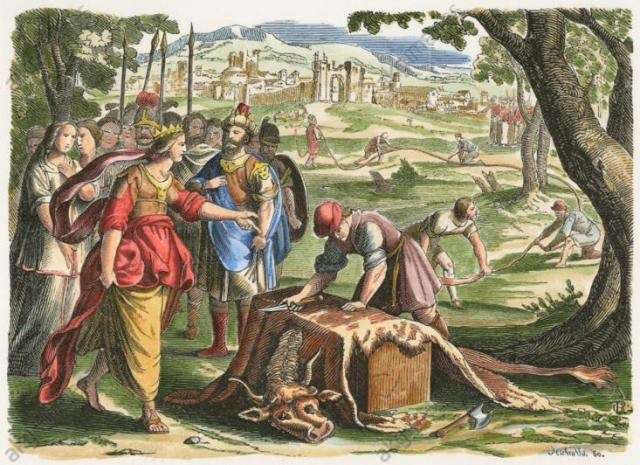
\includegraphics[width=\textwidth]{chapters/050-nebenbedingungen/images/dido.jpg}
\caption{Nach der Gründungssage von Karthago erhielt Königin Dido
vom Numidierkönig Iarbas das Gebiet, das sie mit einer Kuhhaut umspannen
konnte.
Um das Gebiet zu maximieren, lässt Dido die Kuhhaut in schmale Streifen
schneiden.
\label{buch:nebenbedingungen:lagrangemult:fig:dido2}}
\end{figure}
